\chapter*{ステップ1: 環境のセットアップ}
\addtocounter{chapter}{1}
\addcontentsline{toc}{chapter}{ステップ1: 環境のセットアップ}

Dartではパワフルで生産的なツールが提供されています.その中で中心的な位置をしめるものがDart Editorです.Dart Editorは軽量なテキストエディタでDartのアプリケーションの実行,デバッグ,解析が行えます.エディタはDart SDKやDartium\footnote{Dart VMを搭載したChromium}と協調して動作をし,統一された体験を提供します.

\section{目標}

\begin{enumerate}
\item Dart Editorをインストール
\item Editorチームにフィードバックを送信
\item 時計のDartアプリケーションを実行
\item Dartiumについて学ぶ
\end{enumerate}

\section{ウォークスルー}

\subsection{Dart Editorをインストール}

タスク: GoogleIOの時と配布方式が異なるので,記述を変更

To get your environment set up, plug in the provided USB. Open the USB drive and find the \url{editor/} directory inside. Copy over the correct Dart Editor version for your OS/bit combination directory to your machine, and unzip it.

[Image]

Open up the newly unzipped \url{dart/} directory, and double click the executable:

\begin{itemize}
\item DartEditor.app (Mac)
\item DartEditor (Linux)
\item DartEditor.exe (Windows)
\end{itemize}

[Image]

Dart Editorを初めて起動すると,ようこそ画面が表示されます.

\includegraphics{step1/welcome.png}

\subsection{フィードバックを送るボタンを使う}

フィードバックをいただけるとDart Editorチームはとても感謝します.Dart Editorチームにあなたの考え(フィードバック)を知らせる最も簡単な方法はエディタのツールバーの右上にある''Send Feedback''と書かれたボタンを利用することです.

Send Feedbackボタンへマウスを移動しクリックします.

\includegraphics{step1/sendfeedback1.png}

Dart Editorのフィードバックダイアログを利用することで,エディタのチームに直接バグやリクエストを送信することができます.送信していただいた提案はバグレポートや機能リクエストとして登録させていただきます.\footnote{\url{http://dartbug.com}が私達のIssue Trackerです.}

\includegraphics{step1/sendfeedback2.png}

\subsection{時計のサンプルを実行する}

(フィードバックウインドウが開いているときは,閉じてください.)

Dartのアプリケーションを実行してみましょう!

ようこそ画面からClock sampleをクリックします.これをクリックすることで,DartEditorにClock Sampleがコピーされ,新しいプロジェクトがセットアップされます.

\includegraphics{step1/clocksample1.png}

ヒント: ようこそ画面が見つかりませんか? Toolsへ移動して,Welcome Pageをクリックすることで再度表示することができます.

\includegraphics{step1/clocksample2.png}

ファイルビューではClock Sampleのすべてのファイルが表示されています.そこにはDartファイルはもちろん,アプリケーションをホストするHTMLファイル,また,すべてのイメージやCSSも同様に含まれています.clock.dartが''clock''ライブラリを定義しているDartファイルです.そして,そのファイルがこのサンプルのmain()関数を含んでいます.clock.dartファイルはエディタに自動的に開かれます.

\includegraphics{step1/clocksample3.png}

clock.dartファイルが選択されて,ハイライトされていることを確認してください.DartエディタのRunボタンを押してください.このボタンを押すことでDartiumをロードし,アプリケーションが起動され,clock.htmlファイルをDartiumが開きます.

\includegraphics{step1/clocksample4.png}

Clock sampleアプリケーションがDartiumの中で動いています.おめでとうございます!初めてのDartアプリケーションが起動しました!

\includegraphics[width=13cm]{step1/clocksample5.png}

\subsection{Dartium}

DartiumはDart仮想マシンを組み込んだChromiumです.DartはJavascriptへコンパイルしますが,Dartアプリケーションをブラウザの中で直接実行することで,編集,再ロードの開発のサイクルをスピードアップすることができます.

ClockがDartiumで動作していることを確かめるために,ブラウザで右クリックをして,"Inspect Element"を選択してください.

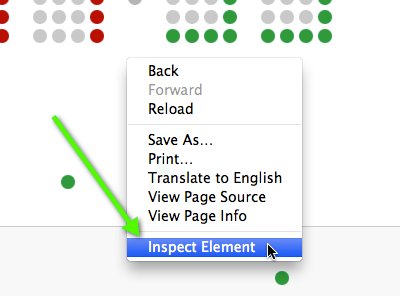
\includegraphics{step1/dartium_img1.png}

Elementsタブがデフォルトで選択されていると思います.clock.dartは実行中のスクリプトとしてリストにあるはずです.

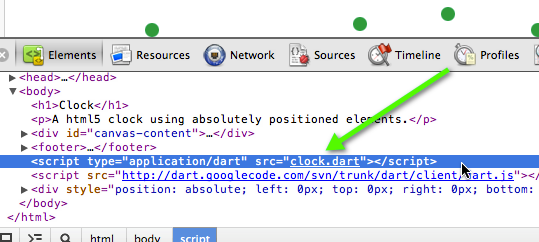
\includegraphics{step1/dartium_img2.png}

\subsection{Dartエディタを利用してのデバッグ}

DartiumでDartを直接実行する場合,エディタはDartアプリケーションのデバッグをサポートします.clock.dartにあるupdateTime()メソッドの中のsetDigits()への初めての呼び出しの位置(66行目)のエディタの左端をダブルクリックすることでブレークポイントを設定します.ブレークポイントを設定した後(小さな青いドットが見えるかと思いますが),Runボタンを再びクリックします.

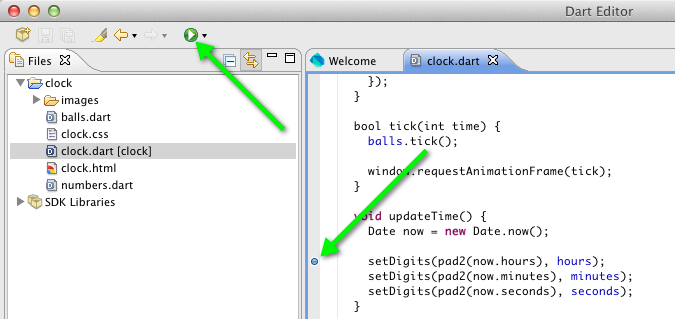
\includegraphics{step1/debug_img1.png}

プログラムが対しして,DebuggerビューがDartエディタの中で開かれます.デバッガかr漁ることなく,プログラムを続けるには,Resumeボタンをクリックします(Debuggerビューにある緑色の矢印です).updateTime()メソッドは1000msごとに呼び出されます.したがって,1秒以内に再び,ブレークポイントに到達することでしょう.

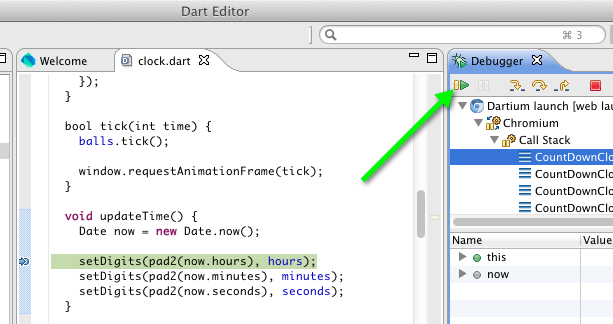
\includegraphics{step1/debug_img2.png}

右側のDebuggerビューを利用することで,どのプロセスが実行されているか,また,ブレークポイントのスコープにおいての値を見ることができます.nowフィールドにマウスをホバーさせると,値がツールチップに表示されることでしょう.

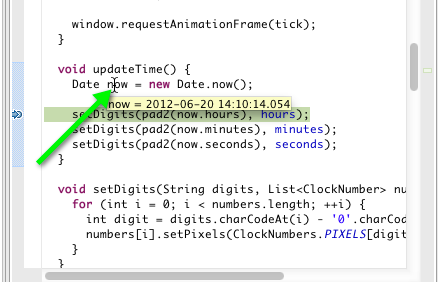
\includegraphics{step1/debug_img3.png}

デバッガを終了させるためには,Debuggerビューの赤色の正方形をクリックします.これを押すことでアプリケーションも同様に停止します.

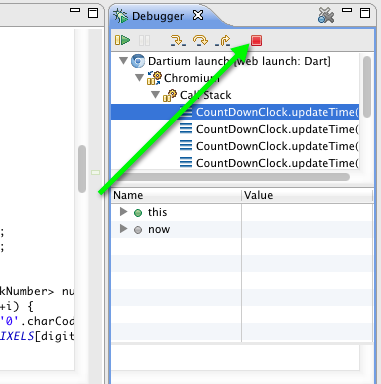
\includegraphics{step1/debug_img4.png}

\section{上級編}

他のサンプルについても読み込んで起動してみましょう.
Clockサンプルにおいて,ボールの速度や重力を変えてみましょう.
balls.dartの12行目から117行目から始めましょう.
もっと多くのブレークポイントを設定して,variablesを開いて値を見てみましょう.

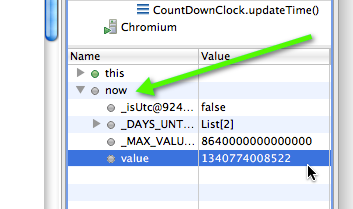
\includegraphics{step1/advanced.png}

\clearpage
